\chapter{Molecular Biology}
Here in this chapter, I will be covering the basics of the relevant molecular biology concepts. This chapter will serve as a reference for the biological claims throughout the document, as well as the foundation for the review chapters of my thesis.

\section{Molecular Mechanism of Angiogenesis}

Blood vessels and the vascular structure are formed by the differentiation of the cells in the mesoderm layer during the embryo development (the layer which also give rise to blood cells, kidney, liver, connective tissue, etc.) \cite{Alberts2002}.

\subsection{A Brief Anatomy of Vessels}
Endothelial cells line all of the vessels. Blood vessels (like the arteries and the veins that are the largest vessels of the body) have a thick and tough wall of connective tissue with several layers of smooth muscles. The wall is lined by a very thin layer of endothelial cells (i.e. the endothelium) separated from the outer surrounding layers by basal lamina \cite{Alberts2002}. It is worth noting that the amount of connective tissue and smooth muscle depends on the diameter of the blood vessel as well as its function, \textbf{but the endothelial lining is always present}. In the finest branches of the vasculature (i.e. capillaries and sinusoids) the wall is just made up of endothelial cells and basal lamina. One of the major roles of the endothelial cells is to control to transport of material in an out of the bloodstream.

A study of embryo development reveals that the even larger vessels (like arteries and veins) start developing from smaller vessels that has only endothelial cells and basal lamina. The connective tissue, smooth muscles and pericytes are added later on, by the signaling from endothelial cells. In particular, the recruitment of pericytes are driven by PDGF (platelet driven growth factor) secreted by the endothelial cells.




\begin{figure}[h!]
	\centering
	% First bottom figure, occupying the left half
	\begin{minipage}{0.4\textwidth}
		\centering
		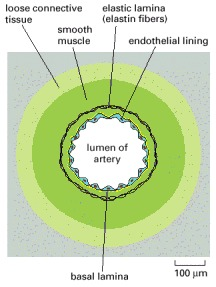
\includegraphics[width=\textwidth]{images/AnatomyOfVessel.jpg}
		% Optional caption for the first bottom image
		% \caption{Caption for the first bottom image.}
		% \label{fig:bottom-left-image}
	\end{minipage} % Space between the two bottom figures
	% Second bottom figure, occupying the right half
	\begin{minipage}{0.4\textwidth}
		\centering
		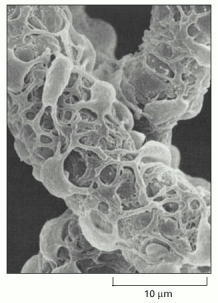
\includegraphics[width=\textwidth]{images/perycitesForVascular.jpg}
		% Optional caption for the second bottom image
		% \caption{Caption for the second bottom image.}
		% \label{fig:bottom-right-image}
	\end{minipage}
\end{figure}
\vspace{-15pt}
\begin{figure}[h!]
	% Top figure spanning the whole width
	\centering
	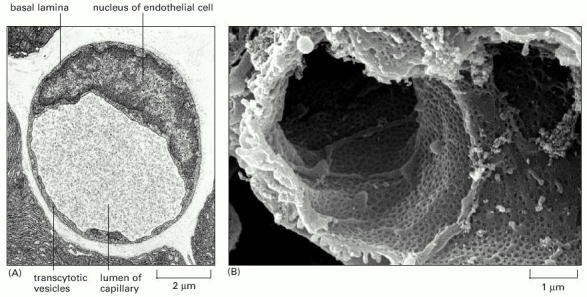
\includegraphics[width=0.8\textwidth]{images/ElectronMicroscopeOfVessel.jpg}
	% Optional caption for the top image
	\caption{\textbf{Figure Top Left:} This figure shows the anatomy of a large vessel, like vein or arteries. Note that smaller vessels, like capillaries as well as sinusoids consists of only endothelial cells and basal lamina, except for some scattered pericytes wrapped around the walls (see figure Top Left). \textbf{Figure Top Right:} Electron micro graph showing small pericytes wrapped around small blood vessels. \textbf{Figure Bottom Left:} A capillary that its wall consists of only endothelial cell and basal lamina. \textbf{Figure Bottom Right:} Electron micro graph showing a cross section of small capillary in pancreas. All of the figures are from \cite{Alberts2002}}

\end{figure}
\FloatBarrier

Also, the following figure summarizes the cross section of different types of vasculature.
\begin{figure}[h!]
	\centering
	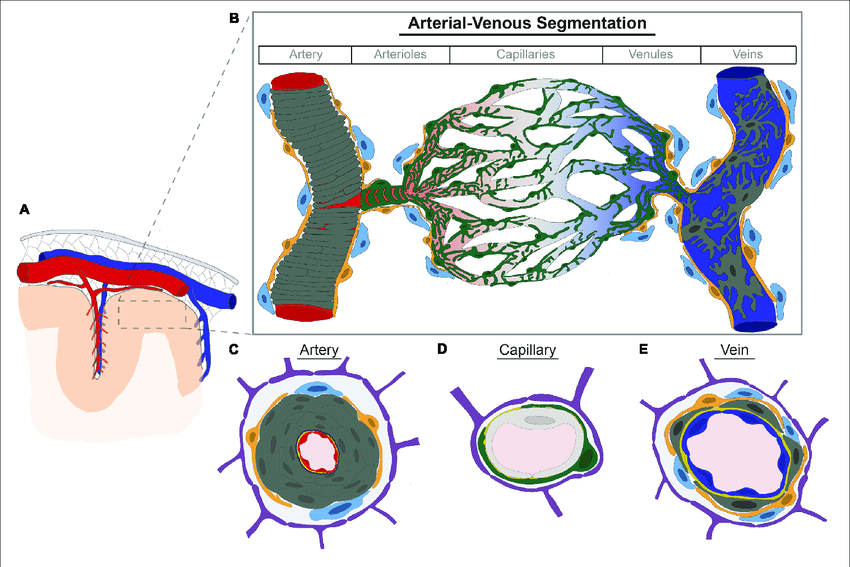
\includegraphics[width=0.8\textwidth]{images/CrossSectionOfVessels.png}
	\caption{The cross section of vessels in the form of arteries, capillaries, and vein. Note the single lining of the endothelial cells for the capillary.}
\end{figure}




\subsection{Molecular Biology of Vascular Structure}

New vessels in the adults originate as capillaries, which sprout from the existing small vessels. Endothelial cells on the arterial and venous side of the developing networks of vessels differ in their surface properties. In the embryo at least, the plasma membrane of the arterial cells contains trans membrane protein ephrine-B2, while the membrane of the venous cells contain the corresponding receptor protein Eph-B4, which is a receptor tyrosine kinase. These molecules mediate a signal delivered at sites of cell-cell contact, and they are essential for the development of a properly organized network of vessels. One suggestion is that they somehow define the rules for joining one piece of growing capillary tube to another \cite{Alberts2002}.


\begin{observation}
	The difference in the surface properties of endothelial cells on the arterial and venous side of the developing networks of vessels control the rate an which one piece of growing capillary tube joins another. This becomes very interesting if we consider it along the observations in \cite{Koery2024}. They observed that the blunt-ended capillaries with small diameter are more susceptible for degradation after irradiation. And since the presence of blunt-ended vessels with small diameter increase the flow resistance of the network, pruning these branches ``normalizes'' the blood flow, hence increase the perfusion after irradiation.
\end{observation}





\subsubsection{Steps involved in angiogenesis}
Individual endothelial cells responds to the signals produced by the organ that they invade. The signal is complex, but the main part of the signal is vascular endothelial growth factor (\textbf{VEGF}) (which is a distant relative of platelet driven growth factor (\textbf{PDGF})). The control on the production of VEGF is through its mRNA stability and its rate of transcription. Under a low oxygen concentration, the  intracellular concentration of an active form of gene regulatory protein called \textbf{hypoxia inducible factor 1 (HIF-1)} increases. HIF-1 stimulates the transcription of VEGF gene (and the production of other genes that are needed when the oxygen supply is low). When the VEGF protein is secreted, it is then diffuses through the tissue and acts on nearby endothelial cells.

Endothelial cells that are to form a new capillary, grow out from the side of an existing capillary by forming long pseudopodia pioneering the formation of new capillary sprout that hallows out to form a tube. This process continues until the sprout encounters another capillary, where they merge. In the tumor micro environment, The growth rate of tumor increases abruptly as soon as the vessels reach it. 

There are two general balancing forces acting on the angiogenesis
\begin{itemize}
	\item Inhibitors:
	\begin{itemize}
		\item endostatin
		\item angiostatin
		\item thrombospondin
	\end{itemize} 
	\item Angiogens
	\begin{itemize}
		\item VEGF: Vascular Endothelial Growth Factors.
		\item bFGF: Basic Fibroblast Growth Factor.
		\item PDGF: Platelet Driven Growth Factor.
	\end{itemize}
\end{itemize}
\FloatBarrier


\subsubsection{The Response of Endothelial Cells to VEGF}
The response of endothelial cells to VEGF has four components. First, they produce proteases to digest through the basal lamina of the parent vessels. For the second step, they migrate towards the source of VEGF, and for the third step they proliferate. Finally, they form hallow tubes. It is worth mentioning that VEGF stimulates endothelial cells selectively, while other angiogens, like fibroblast growth factor stimulates other cell types as well. The following figure summarizes these steps.

\begin{figure}[h!]
	\centering
	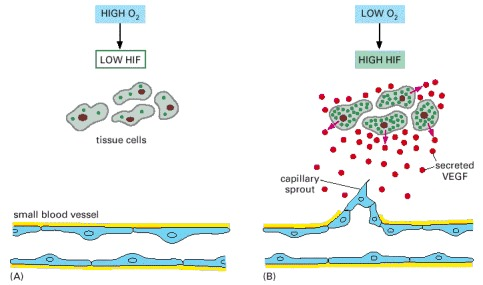
\includegraphics[width=0.8\textwidth]{images/endothelialResponseToVEGF.jpg}
	\caption{A summary of the response of the endothelial cells to VEGF.  Under low oxygen concentration, the intracellular concentration of HIF-1 increases. This gene regulatory protein in turn increases the transcription of VEGF protein. Then VEGF diffuses through the tissue and stimulates the endothelial cells lining the vessels. Figure is from \cite{Alberts2002}.}
\end{figure}


\subsubsection*{Controlling Capillary Joining Process}
In the following text from \cite{Alberts2002}, there is some vague hints about the mechanisms that are controlling capillary joining to each other


\begin{quote}
	Observations such as these reveal that endothelial cells that are to form a new capillary grow out from the side of an existing capillary or small venule by extending long pseudopodia, pioneering the formation of a capillary sprout that hollows out to form a tube (Figure 22-25). This process continues until the sprout encounters another capillary, with which it connects, allowing blood to circulate. Endothelial cells on the arterial and venous sides of the developing network of vessels differ in their surface properties, in the embryo at least: the plasma membranes of the arterial cells contain the transmembrane protein ephrin-B2 (see Chapter 15), while the membranes of the venous cells contain the corresponding receptor protein, Eph-B4, which is a receptor tyrosine kinase (discussed in Chapter 15). These molecules mediate a signal delivered at sites of cell-cell contact, and they are essential for the development of a properly organized network of vessels. One suggestion is that they somehow define the rules for joining one piece of growing capillary tube to another.

\end{quote}

\subsubsection*{Formation of tube structures by endothelial cells}

\begin{figure}[h!]
	\centering
	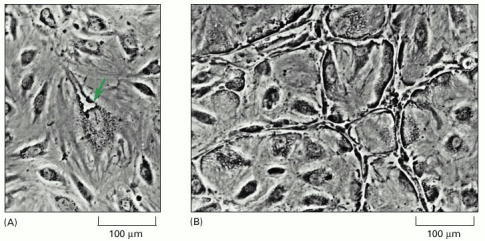
\includegraphics[width=0.8\textwidth]{images/hallowStructureEndothelialCells.jpg}
	\caption{The endothelial cells, when supported by suitable growth medium and signals, start to form hallow structure, that do not contain any blood, and not fluid passes through them. This indicates that the no mechanical trigger (i.e. pressure) is required to form the hallow structure for the new vessels. Image from \cite{Alberts2002}.}
\end{figure}

It was one of my main concerns that what is the process in which a single lining of endothelial cells following a tip cell forms a hallow tube (i.e. vessel). The following text from \cite{Alberts2002} explains this clearly. This process has also been described in \cite{angiogenesisYoutube}.


\begin{quote}
	Experiments in culture show that endothelial cells in a medium containing suitable growth factors will spontaneously form capillary tubes, even if they are isolated from all other types of cells (Figure 22-26). The capillary tubes that develop do not contain blood, and nothing travels through them, indicating that blood flow and pressure are not required for the initiation of a new capillary network. Endothelial cells in culture spontaneously develop internal vacuoles that appear to join up from cell to cell, giving rise to a network of capillary tubes. These photographs show successive stages in the process.
\end{quote}






\section{Biological Assays to Study Angiogenesis}

\subsection{Corneal Micropocket Assay}
This is one of the simple and reproducible assays to study angiogenesis in a eye. The process involves introducing growth factors in the eye ball of mouse, and then letting the vascular network to form. This is a video from JOVE explaining the details of the protocol \citep{conealMicroPocketAssayJOVE}



\section{Some Histology} 

In short, histology is the study of the animal tissue in the microscopic scale (which is also known as the microscopic anatomy or micro anatomy). Studying different types of animal tissue falls in the realm of histology.

\noindent There are four types of animal tissue 
\begin{enumerate}[(i),noitemsep]
	\item Epithelium
	\begin{itemize}
		\item squamous: endothelial lining of the vascular structure is of this type.
		\item cuboidal
		\item columnar
	\end{itemize}
	\item Muscle tissue
	\begin{itemize}
		\item smooth muscle
		\item skeletal muscle
		\item cardiac muscle
	\end{itemize}
	\item Connective tissue
	\begin{itemize}
		\item cartilage
		\item bone
		\item blood
		\item lymph
		\item hemopoietic
	\end{itemize}
	\item Nervous tissue
	\begin{itemize}
		\item central nervous system
		\item peripheral nervous system
	\end{itemize}
\end{enumerate}

Among this list of the four basic types of the animal tissue, we will focus on the Epithelium.

\subsection{Epithelium}
Epithelium forms continuous sheets of cells that line internal surfaces and cover the external surfaces of the organs. A \textbf{basement membrane} separates an epithelium from the underlying connective tissue. 


\begin{figure}[h!]
	\centering
	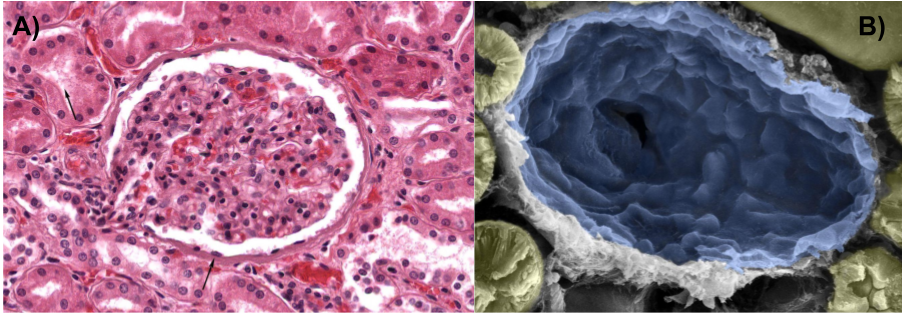
\includegraphics[width=0.8\linewidth]{images/histologySquamousEpithelial}
	\captionsetup{width=0.9\textwidth} 
	\caption{A) A microscopic image of renal corpuscle that contains a glomerulus (a tuft of capillaries) surrounded by Bowman's capsule. The interior of the capsule, is lined with a simple squamous epithelial that rests on a thick basement membrane. The only part of these cell visible is their nuclei bulging into the interior. B) Scanning electron microscope of renal corpuscle that its glomerulus is removed. The simple squamous epithelial can be seen in blue (borders of individual cells are not visible). Both images are from histologyguide.com.   }
	\label{fig:histologysquamousepithelial}
\end{figure}
\FloatBarrier

\begin{figure}[h!]
	\centering
	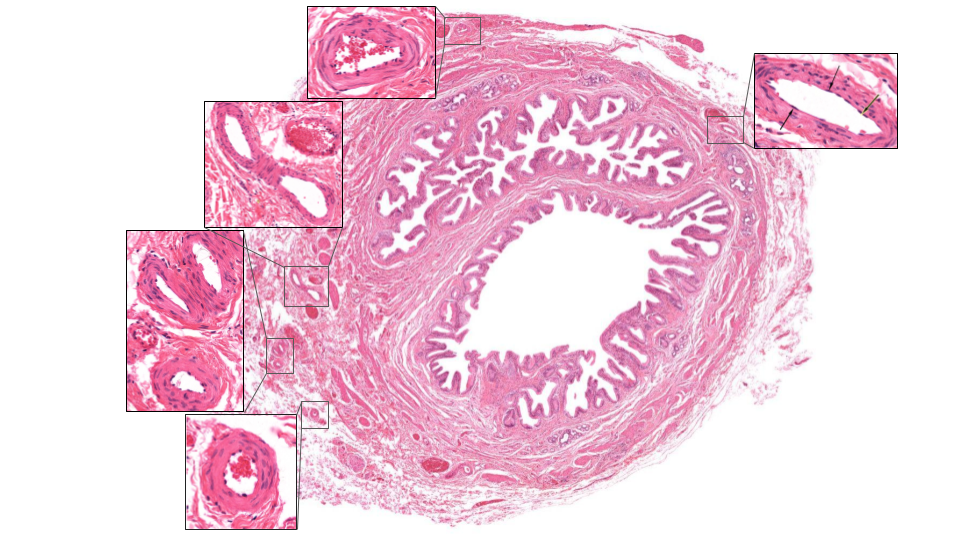
\includegraphics[width=0.8\linewidth]{images/bileDuct-SquamousEpithelialCells.png}
	\captionsetup{width=0.9\textwidth} 
	\caption{A pathology image of bile duct (the large lumen at the center). There are many blood vessels in the surrounding connective tissue. Blood vessels are lined with simple squamous epithelial. The only par of these cells visible is their flatten nuclei. \textbf{Epithelium that lines blood vessels, heart, and lymphatic vessels is also known as endothelium.}}

\end{figure}


\section{Important Facts}
\begin{itemize}
	\item The over expression of ANG1 (angiopoeiting1) induces vascular remodeling that leads to the formation of vessels with a wider diameter (\cite{Augustin2009}).
	\item  TIE2-mediated EC activation controls the expression of endothelial apelin, which in turn acts in an autocrine manner on EC-expressed G-protein-coupled APJ receptors, the downstream signalling of which contributes to the control of vessel diameter (\cite{Augustin2009,Kidoya2008}).
	\item  Differences in arterio-venous shear stress also control Ang–Tie signalling (\cite{Augustin2009}).
	\item The quiescent EC phenotype is maintained by constitutive ANG1–TIE2 signalling. ANG1 clusters TIE2 junctionally at inter-endothelial cell junctions in trans to transduce survival signals. Differences in arterio-venous shear stress also control Ang–Tie signalling. During the transition from the quiescent to the activated phenotype, ECs liberate their endogenously stored pools of ANG2, and this antagonizes ANG1–TIE2 signalling to facilitate EC responsiveness to exogenous cytokines. As such, the absence or presence of stored ANG2 contributes to the control of the \textbf{adaptive plasticity of the vascular endothelium} (\cite{Augustin2009}).
	\item  Oscillatory flow has also been measured in humans and reported in \cite{Rodgers1984} (\cite{Carr2005}).
	\item Observed oscillation frequencies range up to 240 cycles per minute. High frequency oscillations (greater than 50 cycles per minute) have been attributed to either heart pulse or breathing rhythms. Lower frequency oscillations are thought to be caused by vasomotion. Observed frequencies of vasomotion have been reported to range from 2.7 to 32 cycles per minute.6,23 Recent analysis of RBC velocities and arteriole diameter dynamics by Parthimos et al. suggests, however, that low frequency oscillations may not be solely due to vasomotion. Their analysis demonstrates that two important measures (correlation dimension
	and Lyapunov exponent) of the RBC velocity oscillations
	depends on whether vasomotion is present or not. This indicates that something other than vasomotion is also driving
	the RBC velocity dynamics \cite{Carr2005}
	\item The responses outlined above lead to continued vessel shrinking and eventually to pruning of vessels that are nonfunctional with respect to both convective and diffusive transport. Typically, such vessels have low shear stress and moderate or high oxygen levels and therefore receive a negative net growth stimulus, causing decrease in diameter \cite{Pries2014}.
	\item The need for distribution of capillaries throughout the tissue implies the presence of both short and long flow pathways connecting the feeding arteriole to the draining venule. As illustrated in FIGURE 4, a short pathway has a very high pressure drop per length and thus very high wall shear stress compared with the feeding arteriole from which it branches. On the other hand, the local oxygen partial pressure and metabolic environment of the two segments are similar. Responses to local signals alone would therefore favor growth in the short pathway, generating a functional arterio-venous (A-V) shunt. To avoid such behavior, an additional mechanism is required that signals differences between arterioles supplying a large number of capillaries and those forming short A-V connections. This mechanism must provide transfer of information upstream along arterioles within vascular networks. A similar consideration applies to vessels in the venular network, where information transfer in the downstream direction, from distal to proximal vessels, is necessary. In this case, convective transport of metabolites may provide the needed signals (55, 63). However, upstream information transfer is not so simply explained \cite{Pries2014}.
	\item If the shrinking of a given vessel leads neither to local hypoxia nor to increased wall shear stress, then it receives no increasing growth stimulus and continues to shrink, eventually being pruned \cite{Pries2014}.
	\item Conversely, shrinkage of a vessel that is needed for diffusive transport leads to hypoxia and an increased metabolic stimulus for growth, whereas shrinkage of a vessel that is needed for convective transport leads to increased wall shear stress, also a stimulus for vessel growth. In each case, the resulting negative feedback loop stabilizes vessel diameter \cite{Pries2014}.
	\item Third, angiogenesis, remodeling, and pruning occur in parallel and not as separate processes \cite{Pries2014}.
	\item An interesting prediction of the theory is that this system exhibits hysteresis: the increase in vascular density generated during a period of higher demand is only partially reversed if demand returns to its former level \cite{Pries2014}.
	\item Under steady-state conditions, endothelial cells are relatively quiescent, exhibiting a turnover time in the range of ∼30–300 days (see reference 18,35 of \cite{Pries2014}).
	\item In tumors, the microvasculature is typically seen to be more tortuous and disorganized than in normal tissues. Tumors often show a relatively high proportion of hypoxic tissue, even if the vascular volume and perfusion are relatively high. This hypoxia has important effects on tumor responses to radiation and chemotherapies, generally reducing their effectiveness. Analysis of hemodynamics and remodeling in tumor microvessel networks suggests that poor oxygenation may result from functional shunting, i.e., failure to distribute flow appropriately between short and long flow pathways, as a consequence of impaired conducted responses (55, 56). Such impairment is plausible given that endogenous VEGF levels are typically elevated in tumor tissues and that VEGF has disruptive effects on vascular wall integrity and gap junction function (74) \cite{Pries2014}.
	\item The dense but highly disordered and functionally deficient vascular networks often observed in tumors can be interpreted as the result of excessive angiogenesis combined with weak or defective remodeling and pruning. Similar patterns with increases of vessel density but not perfusion have been reported to result from VEGF overexpression (78) \cite{Pries2014}.
	\item Therefore, understanding the formation of
	vascular networks requires consideration of the integrated processes of angiogenesis, structural adaptation, and pruning \cite{Pries2014}.
	\item These structural adaptations may involve alterations in the dimensions and wall composition of individual vessel segments (remodelling), the growth of new segments (angiogenesis) and the loss of existing segments (pruning)\cite{Secomb2012}.
	\item  in the development of hypertension, inward remodelling accompanied by wall thickening is a typical structural feature \cite{Secomb2012}.
	\item Some experimental references for the vascular remodeling and adaptation: Direct experimental approaches have provided much information about structural remodelling of blood vessels. Ex vivo perfusion systems allow manipulation of haemodynamic conditions and observation of resulting structural changes over periods of hours to days [3–5]. In vivo animal models can be used to observe structural responses to surgical alterations in flow conditions over periods of days to weeks [6–10]. Such experimental approaches have been used to investigate the responses of individual vessels (generally arteries) to mechanical stimuli, including fluid shear stress acting on the endothelial cell layer and circumferential and axial stresses acting on the wall, and to metabolic and pharmacological stimuli \cite{Secomb2012}.
	\item Early theories of structural adaptation assumed that the diameter of each segment is controlled so as to achieve a target level of the wall shear stress [18,19] \cite{Secomb2012}.
	\item However, analyses of microvascular networks in the rat mesentery [22] showed a systematic increase in wall shear stress with intravascular pressure from the venules to the arterioles. Such behaviour was incorporated in the model by assuming a pressure-dependent set point for wall shear stress. This implies that venous vessels are larger than corresponding arterial vessels carrying the same blood flow. Another consequence is that the pressure drop is much larger in the arterioles than in the venules, and capillary pressure is much lower than arterial pressure \cite{Secomb2012}.
	\item Analysis of the model under the assumption that diameters respond only to the haemodynamic signals of pressure and wall shear stress shows that parallel flow pathways are unstable (fig. 2A) [19]. Furthermore, this assumption neglects the obvious need for network structure to respond to metabolic needs. Introduction of a signal dependent on local oxygen level (fig. 1B) provides a metabolic response and can be shown to stabilize parallel pathways (fig. 2B). \cite{Secomb2012}
	\item Mechanical parameters such as tissue elasticity, viscosity and friction can also specify time and length scales of morphogenetic processes (Fig. 1a). For instance, the length scale of stress propagation, the so-called hydrodynamic length, depends on the relative contribution of viscosity and friction within a cell [30] or a tissue. Viscosity can also define rates of deformation upon a given mechanical stress. The ratio between the viscous modulus and elastic modulus defines the Maxwell time, that is, the time above which deformations become irreversible, typical of a viscous response[31]. Mechanics can thus direct morphogenesis in a manner similar to biochemical information. For instance, dissipation of a localized stress by friction can generate gradients of stress similar to those better known for biochemical gradients of morphogens [32,33] \cite{Collinet2021}
	\item We delineated two idealized and distinct modalities of information flow during morphogenesis. Programmes specify deterministically and hierarchically all operations required for the development of a shape. Programmed morphogenesis results explicitly and predictably from the spatially organized initial conditions, a pre-pattern, and relies upon deterministic rules. For instance, a genetically encoded morphogen gradient specifies a battery of downstream decisions that themselves dictate mechanical states in cells such as cell contractility. By contrast, self-organization is characterized by the emergence of ordered structures from a purely homogeneous initial state. It relies on stochastic rules, local activity associated with molecular motors and dissipation of elastic energy, driving irreversible deformation and amplification of local activity via feedbacks that operate across scales. Thereby, the system transits to a steady state that minimizes its free energy \cite{Collinet2021}.
	\item Programmes are usually hard-wired and exhibit redundancy, such that they are mostly insensitive to genetic perturbations. However, once affected, for example by a mutation, they cannot be repaired to generate the expected shape because of the absence of feedbacks and a strict dependency on initial conditions, which may be lost as morphogenesis proceeds. By contrast, owing to their internal feedbacks, rapid dynamics and insensitivity to initial conditions, self-organized systems can reform after complete perturbations and constantly adapt to a changing environment. Thus, programmes may be most suited to robustly guide a few critical steps of morphogenesis where failing to properly time or position singular shape changes of the tissue may affect the entire subsequent steps of the morphogenesis, such as during embryo gastrulation or the specification of primary sulci in the developing brain cortex \cite{Collinet2021}.
	\item The energy minimisation formalism used here is consistent with Murray’s law. In Murray’s approach, it is assumed that there are two contributions to the energy cost of maintaining the flow: the power required to overcome viscous drag forces and the metabolic cost of maintaining the network structure, which is proportional to its volume \cite{Almeida2022}.
	\item Animals and plants may benefit from loop structures in many ways. For example, loops are important in mitigating damages of networks [3] and optimizing energy consumption with fluctuating flow distributions [3,4]\cite{Hu2013}.
	\item biological transport networks are thought to have undergone a process of gradual optimization through evolution [1], culminating in organizational principles such as Murray’s law [2–4]. A particular class of such networks that minimizes flow resistance under biologically relevant constraints has been studied to reveal a wealth of phenomena such as phase transitions [5,6], the interdependence of flow and conduit geometry [7], and predictions about allometric scaling relations in biology [8]. When the optimization models are generalized to require resilience to damage or to consider fluctuations in the load, optimal networks reproduce the reticulate network patterns observed in biological systems [9,10]. The optimality principles that often determine these networks also appear in nonbiological context, e.g., river basins [11,12], and are relevant for man-made systems such as gas or sewage pipe networks [13,14] \cite{Ronellenfitsch2016}.
	\item The topology of such efficient networks is characterized by the tendency to reuse the same edge to supply large parts of the network, as opposed to directly connecting each node to the source. This is reflected in the mean number of edges between two bifurcations (the mean branch length). Efficient networks tend to exhibit fewer nonbranching nodes [Fig. 3(c)]. Temporally fluctuating sources (similar to [27]) during the adaptive process can produce loops [33], reminiscent of real reticulate biological networks. In addition, variable branching angles [7], growth anisotropies, and steric effects [33] may also play a role \cite{Ronellenfitsch2016}.
	\item Growth effectively reduces the dimension of the evolutionary search space to two parameters that can be used to explore the energy landscape \cite{Ronellenfitsch2016}.
	\item Natural and man-made transport webs are frequently dominated by dense sets of nested cycles. The architecture of these networks, as defined by the topology and edge weights, determines how efficiently the networks perform their function. \cite{Modes2016}
	\item For many purposes, e.g., when analyzing blood flow in arteries, the dependence of viscosity on shear rate can be neglected and blood can be treated as a Newtonian fluid as defined above \cite{Secomb2021}.
	 the apparent viscosity in large vessels matches the in vitro result, but the apparent viscosity is substantially higher than the in vitro estimate in smaller vessels. For example, the estimated apparent viscosity in a $7\mu m$ capillary at hematocrit $45\%$ is about $8.4\mu_p$, almost seven times higher than would be expected based on data from glass tubes.
	 \item An important implication of the existence of the endothelial surface layer is that the endothelial cell membrane does not experience a significant level of fluid shear stress due to plasma flow over its surface. Instead, shear stress is transmitted to the endothelial cells via the attachment points of the macromolecules that anchor the ESL, including syndecans and glypicans [23, 24]. Being transmembrane proteins, these molecules may in turn transmit the shear stress to the internal cytoskeleton, consistent with an important role for the cytoskeleton in mechanotransduction of shear stress [25, 26] \cite{Secomb2021}.
	 \item However, when the flow of blood is considered, additional complexity arises because blood is a concentrated suspension of cells, whose dimensions are comparable to microvessel diameters. As mentioned earlier, red blood cells show a tendency to migrate away from microvessel walls. The fluid mechanical mechanisms underlying this behavior depend on the deformability of the cells and on the fluid dynamical interactions of cells with the walls and are only partially understood [18, 28,29,30,31,32,33]. The distribution of red blood cells across the vessel cross-section affects the distribution of hematocrit in each branch when the flow reaches a diverging microvascular bifurcation [34], and the theoretical understanding of this phenomenon is a challenging problem in the low Reynolds number flow [35,36,37] \cite{Secomb2021}.
	 \item Transport of oxygen is a critical function of the circulation. Being a non-polar molecule, it has relatively low solubility in water and in tissue \cite{Secomb2021}.
	 \item Therefore, it must be delivered by convective transport within such a distance of all cells that require oxygen. This requires a dense network of tiny vessels throughout the tissue. On the other hand, viscous resistance to blood flow is very high in vessels with very small diameters. For mechanical efficiency, the vascular system must include hierarchical branching structures feeding the microvessels, such that convective transport over larger distances can be achieved by vessels with larger diameters and lower resistance to flow. In effect, the vascular system must solve a complex patterning problem, generating a structure in which a dense meshwork of capillaries is combined with a hierarchical structure of arteries, arterioles, venules, and veins of varying lengths and diameters so that all parts of the tissues are adequately supplied with blood flow [40] \cite{Secomb2021}.
	 \item A quick anatomy: Blood vessels are mainly formed by endothelial cells (ECs) and mural cells (MCs). ECs are responsible for the exchange and barrier functions of the vascular network. MCs, which are in close contact with the ECs, contribute to vessel stability. Vessels with a large caliber (arteries and veins) are sheltered by vascular smooth muscle cells (vSMCs) while capillaries are covered by pericytes (PCs) (Potente and Mäkinen, 2017; van Dijk et al., 2015) \cite{Ouarne2021}.
	 \item lood vessels develop by distinct mechanisms (Semenza, 2007). First, vasculogenesis forms the primary vascular plexus by a de novo production of ECs from the mesoderm (Kolte et al., 2016; Potente and Mäkinen, 2017). Then, vascular networks grow through angiogenesis, a process responsible for the formation of new blood vessels from pre-existing ones (Potente and Mäkinen, 2017) \cite{Ouarne2021}.
	 \item Angiogenesis can occur by two different mechanisms: i) sprouting angiogenesis, characterized by the expansion of pre-existing vascular networks into a web of interconnected capillaries; and ii) intussusceptive angiogenesis, characterized by the formation of an intussusceptive pillar, splitting and remodeling of blood vessels \cite{Ouarne2021}.
	 \item Vessel pruning plays a crucial role in optimizing blood flow within immature vascular networks, contributing to their hierarchical organization. This process involves the selective removal of superfluous or non-perfused vessels. Unlike vascular involution, vessel pruning does not rely on endothelial cell (EC) death. Instead, it depends on the migration and rearrangement of ECs in response to blood flow (Fonseca et al., 2020; Potente et al., 2011). In fact, only 5 to 15\% of vessels undergoing pruning contain apoptotic ECs (Franco et al., 2015; Y. Zhang et al., 2018b) \cite{Ouarne2021}.
	 \item This is a dynamic process of structural adaptation and flow regulation that continually adjusts the vessel caliber to compensate for heterogeneity, leading to a flow redistribution according to metabolic needs to ensure adequate tissue oxygenation (Roy and Secomb, 2020) \cite{Ouarne2021}.
	 \item Vascular quiescence stabilizes the vascular network by halting its development, allowing endothelial cells (ECs) to specialize and mural cells (MCs) to mature into their specific organ functions. During quiescence, ECs stop proliferating and migrating (Ricard et al., 2021), creating a balanced state supported by mature MCs. However, this equilibrium is not permanent; quiescence can be disrupted during various physiological processes, such as pregnancy and the menstrual cycle (Carmeliet, 2005; Ricard et al., 2021), as well as in pathological conditions (see Section 6) \cite{Ouarne2021}.
	 \item where $ \rho $ is the “resistivity”, which is supposed to be the same for all the pipes. For $ m = 1 $, the flow in each channel is pluglike (e.g., electric current in metallic wire, liquid flow in porous conduct,…), while for $ m=2 $, the flow is Poiseuille-like (e.g., laminar viscous flow in pipe)\cite{Durand2006}.
	 \item Therefore, it may be of interest to compare the structure of some natural networks with the results presented in this work. Indeed, it has been already shown in various publications [22,23] that Murray’s law is well satisfied in some appropriate portions of human and animal vascular systems. In that case, the flow profile is nearly Poiseuille-like ($ m=2 $) and the relevant constraint is a fixed total channel volume ($ n=1 $) [22,23] \cite{Durand2006}.
	\item 
	\begin{figure}
		\centering
		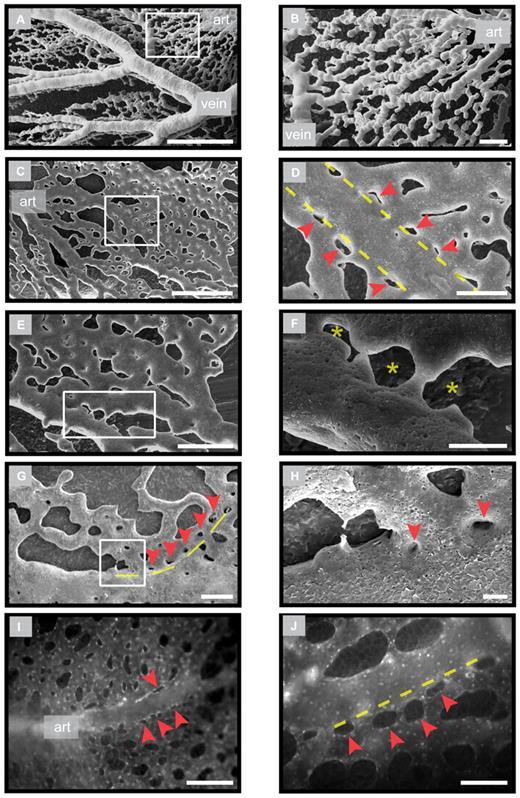
\includegraphics[width=0.5\linewidth]{images/pillarFormationInEmbryoLigation}
		\caption{Splitting angiogenesis (intussusception) in ligation embryos. (A-H) Scanning electron micrographs of vascular corrosion casts of control (A,B) and ligation (C-H) chicken embryos. (A) Low magnification of the normal vasculature. The boxed region is shown at higher magnification in B. Splitting angiogenesis is not apparent. (C) Micrograph of ligation embryo showing extensive pillar formation. (D) Magnification of the boxed region in C, showing rows of pillars (red arrowheads) delineating the future arteriolar segment (dashed line). (E,F) Overview (E) and detail of the boxed area (F) showing fusion of pillars leading to segregation of the capillaries (asterisks). (G,H) Another example showing the advanced splitting by pillars (arrowheads); rows of pillars align (dashed line) and subsequent fusion will lead to separation of the feed vessel from the surrounding capillary plexus. (I,J) Fluorescent labeling of endothelial cells in vivo shows pillar formation (arrowheads) in distal arterioles and the connected capillary network. art, artery. Scale bars: 500 μm in A,C; 200 μm in E; 100 μm in B,D,G; 50 μm in F; 20 μm in H; 30 μm in I,J. Figure is from \cite{Buschmann2010}}.
	\end{figure}
	
\end{itemize}


